\section{Sample Size Calculation}

\begin{frame}{}
  \begin{center}
    {\bf Part I -- Introductio and Motivation}
  \end{center}
\end{frame}

\subsection{Introduction}

\begin{frame}{Lecture Outline}

  In this course we talked several times about the necessity
  of collecting {\bf a sample}: A set of (multiple) observations
  that are used to calculate the value of interest.
  \bigskip

  However, up until now we have avoided talking about {\bf how big} this sample should be. This is the topic of today's lecture.\bigskip

  \begin{itemize}
    \item What is sample size?
    \item Why do we need to worry about it?
    \item What factors influence the choice of sample size?
    \item How to calculate the desired sample size?
  \end{itemize}

\end{frame}


\subsection{Motivation}

\begin{frame}{Why take samples?}{Review: Noise Factors}
  As we discussed before, the result of an experiment is affected by several factors, some of which are unknown, or difficult to control.\bigskip

  Because of these {\bf Noise Factors}, sometimes there will be a small variance in the result of repeated experiments. To measure this variance, and take it into account for our analysis, we repeat the experiment several times, and gather those repetitions into a {\bf sample}.\bigskip


  \begin{columns}
    \column{0.2\textwidth}
      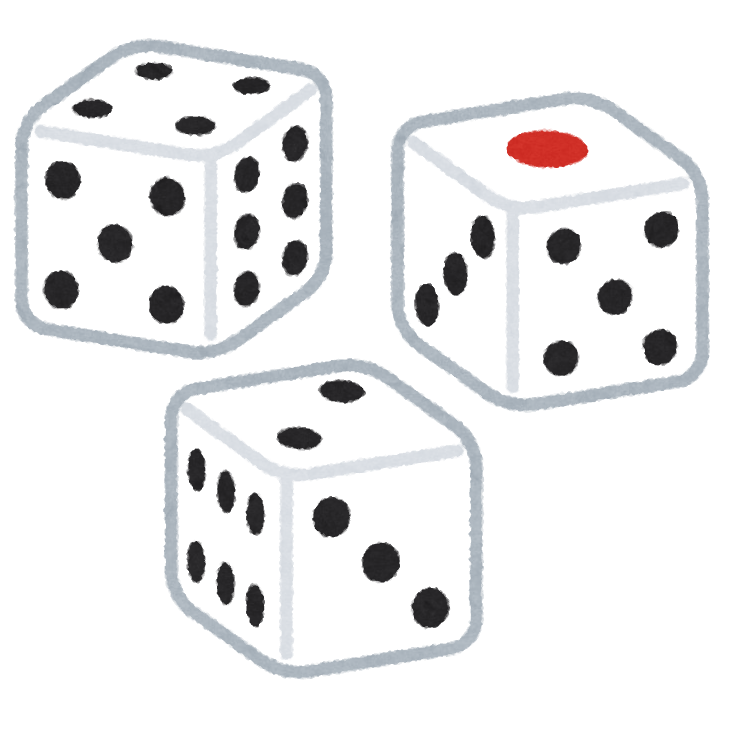
\includegraphics[width=\textwidth]{../img/irasutoya_dice}
    \column{0.8\textwidth}
      {\bf For example:} The true mean of throwing three dice and adding their values is {\bf 10.5}. However, every time we throw the dice, the result will be a bit different.
  \end{columns}
\end{frame}

\begin{frame}[fragile]{Why take samples?}{Sample size and estimation error}

  \begin{columns}
    \column{0.2\textwidth}
      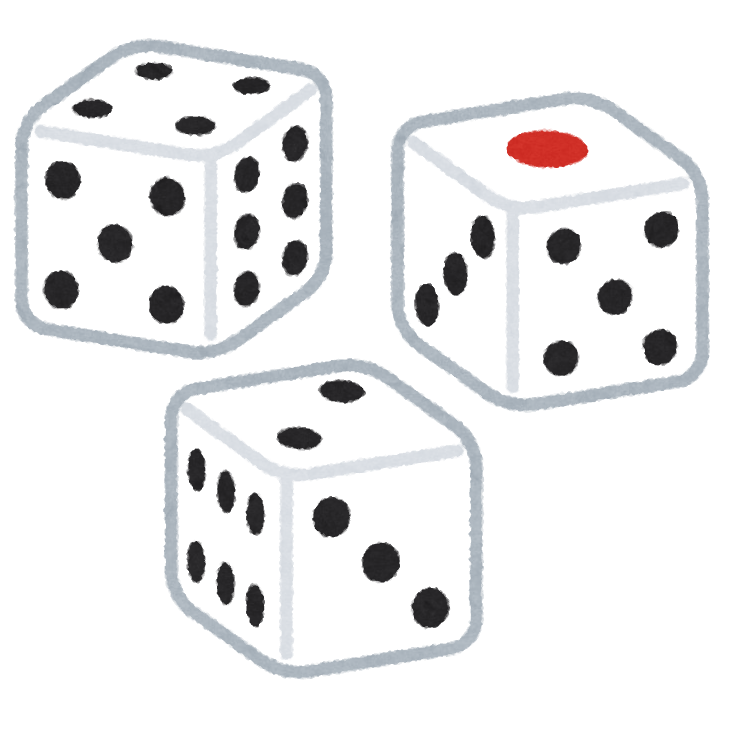
\includegraphics[width=\textwidth]{../img/irasutoya_dice}
    \column{0.8\textwidth}
      If we want to estimate the mean value of a noisy process (for example, the mean of three dice), we can observe the process multiple times (a sample), and take the average of the sample values.\bigskip

      As the sample size gets larger, the sample error \alert{usually} gets smaller. {\bf However, the noise of the original process does not change!}
  \end{columns}
{\smaller
\begin{verbatim}
> sample_2 <- replicate(2, sum(sample(6,3)))
9 6
> sample_5 <- replicate(5, sum(sample(6,3)))
11 10  9 11 12
> sample_10 <- replicate(10, sum(sample(6,3)))
9 11 12 11  7  9 14 11 13 10
> mean(sample_2)          #    7.5       > sd(sample_2)          # 2.12
> mean(sample_5)          #   10.6       > sd(sample_5)          # 1.14
> mean(sample_10)         #   10.7       > sd(sample_10)         # 2.05
\end{verbatim}}
\end{frame}

\begin{frame}{Why take samples?}{}

Larger sample sizes help us isolate the error related to the {\bf noise of the
process}. This has an influence on:\bigskip

\begin{itemize}
  \item Size of the confidence interval of the estimator;
  \item Confidence of statistical tests;
  \item Power of statistical tests;
\end{itemize}\bigskip

This is why we are interested in having "big enough" sample sizes.
\end{frame}

\begin{frame}{Is "as much as possible" the answer for sample size?}

  From what we talked until now, it is natural to think that "more observations is always better". In general, it is a good idea to have a large sample size, but
  there are other things that need to be considered:\bigskip


  \begin{itemize}
    \item Many experiments have a cost associated with obtaining each observation. So large sample sizes result in large experimental cost.\medskip

    \item Some experiments require materials or conditions that are hard to obtain
    (for example, interviews);
  \end{itemize}\bigskip

  The increase in sample size has \alert{diminishing returns} in terms of confidence and power of tests. So, sometimes the cost of collecting more observations is higher than the benefit of those observations.
  \medskip

  So, what is the appropriate sample size for a given experiment?
\end{frame}

\begin{frame}{What is a good sample size?}
  For the choice of sample size, you usually take three things in consideration:
  \bigskip

  \begin{itemize}
    \item The cost of the experiment;
    \item The desired confidence ($\alpha$, Confidence interval size);
    \item The desired power ($\beta$)
  \end{itemize}\bigskip
\end{frame}

\subsection{Fixed Sample Size}

\begin{frame}{Calculating Sample Size: When you don't have a choice}

When an experiment is constrained by budget (not enough time,
not enough money, etc), we might not have a choice of sample size.\bigskip

But even if the sample size is fixed by the experimental conditions, it is still
important to calculate the power of the experiment. The result of power
calculation tells us how we should interpret the results of the experiment.\bigskip

To calculate the power of the experiment, we need to first define the minimum
interesting effect size $\delta^*$.
\end{frame}

\begin{frame}[fragile]{Example of power calculation}

Consider an one-sample experiment with the following parameters: Alternate hypothesis is one-sided, sample size is 10, $\delta^*=0.5$, estimate of standard deviation is $\sigma=1$, desired significance $\alpha=0.01$.\medskip

What is the power of this experiment?

{\smaller
\begin{verbatim}
> power.t.test(n = 10, sd = 1, sig.level = 0.01, type = "one.sample",
+              alternative = "one.sided", delta = 0.5)

  One-sample t test power calculation

           n = 10
       delta = 0.5
          sd = 1
   sig.level = 0.01
       power = 0.1654013           <- Power = 0.16 - Very low!
 alternative = one.sided              High chance for false negatives
                                      *For this effect size*
\end{verbatim}}
\end{frame}

\begin{frame}[fragile]{Example of power calculation}{Increasing the power by increasing $\delta^*$}

If we want to increase the power of the experiment, but we cannot increase the
number of observations, we could increase the size of the "minimal difference"
that this test detects. This calculation will tell us what is the minimum difference
that our test will observe.

{\smaller
\begin{verbatim}
> power.t.test(n = 10, sd = 1, sig.level = 0.01, type = "one.sample",
+              alternative = "one.sided", power = 0.8)

   One-sample t test power calculation

            n = 10
        delta = 1.185308         <- When we fix the power and the sample size,
           sd = 1                   the calculation tells us that the minimum
    sig.level = 0.01                effect size becomes "1.18". If the real
        power = 0.8                 effect is less than this, the probability
  alternative = one.sided           of a false negative increases.
\end{verbatim}}
\end{frame}

% %%%%%%%%%%%%%%%%%%%%%%%%%
%
% \begin{frame}{Sample size and Type-II error}
% {Estimating Experimental Power}
%   A strategy for estimating an effective lower bound for the power of a test includes a definition of an \textit{minimally interesting effect} $\delta^*$.
%   \bigskip
%
%   This value must be derived from technical and scientific knowledge about the phenomenon or system under experimentation.
%   \bigskip
%
%   \begin{block}{}
%   \centering It is essential to have a good understanding of the field in which the experiment will be conducted.
%   \end{block}\bigskip
%
%   Once $\delta^*$ is defined, the experimenter can obtain an estimate of the variability of observations (e.g., by a pilot study), which can then be used to obtain an approximate power value for the experiment;
% \end{frame}
%
% %=====

\begin{frame}{Power calculations}{Some considerations}
  Using power calculations, we can obtain the estimation of the Type-II error probability. This gives us a better understanding of the ability of an experiment
  to detect effects of interest.\bigskip

  The statistical test will have lower power for differences smaller than $\delta^*$, but these differences are below the minimally interesting effect; any effect greater than $\delta^*$ will result in a higher power for the test;\bigskip

  This technique is most useful to compute the required sample size for the   experiment.
\end{frame}



\subsection{}
\begin{frame}{}
  \begin{center}
    {\bf Part II -- Sample Size Calculation}
  \end{center}
\end{frame}


\subsection{The magic number "30"}

\begin{frame}{"We repeat each experiment 30 times"}
  We see many papers use this sample size without much explanation.
  \bigskip

  Why 30 repetitions? Is it a good value?
\end{frame}

\begin{frame}{Why 30 repetitions?}
  Remember that the {\bf Central Limit Theorem} (CLT) states that the distribution
  of the "sample mean" estimator becomes closer to normal, as the sample
  $n$ size increases.\bigskip

  When $n > 30$, the CLT holds (the sample mean follows a normal distribution)
  for most cases (except very extreme cases of non-normality). This is important,
  because many test statistics require the assumption of normality.
  \bigskip

  {\bf However!} Other than (potentially) guaranteeing that the estimator
  is a normally distributed random variable, there is nothing special about
  using 30 repetitions.\bigskip

  \structure{In particular, $n=30$ does not guarantee anything about the power or confidence of the experiment, so you still need to perform power calculations! (And you also need to guarantee the other assumptions of the experiment.)}
\end{frame}

%%%%%%%%%%%%%%%%%%%%%%%%%%%%%%%%%%%%%%%%%%%%%%%%%%%%%%%%%%
\subsection{Sample Size Calculation}

% - Sample size calculation
%   - sample size calculation for single sample test

\begin{frame}[fragile]{Sample Size Calculation}{One Sample Testing}

The sample size calculation in related to the power calculation. If we fix
the value of power and $\delta^*$, the calculation will give us the minimum sample size:

{\smaller
\begin{verbatim}
> power.t.test(sd = 1, sig.level = 0.01, type = "one.sample",
               alternative = "one.sided",   power = 0.85,     delta = 0.5)

  One-sample t test power calculation
           n = 47.98044   # <-- Round this value up!
       delta = 0.5
          sd = 1
   sig.level = 0.01
       power = 0.85
 alternative = one.sided
\end{verbatim}}

We need at least 48 observations to detect a one-sided effect of $\delta^* = 0.5$ or more on the mean with a power level of $0.85$.
\end{frame}

%   - sample size calculation for post-hoc multi-sample test
%   - Methods for z tests, methods for post-hoc tests
% - Be careful with sample size calculations:
%   - Pseudo-replication (it is not the sample size the matters, but how you choose it.)
%     - An extreme example: We develop an algorithm to solve optimization problems.
%     - The optimization problems have "Types", "Sub-types", and "Sub-Sub types"
%     - We are interested


\subsection{Sample Size for Two Means}

%% TODO: Add the experimental context here
\begin{frame}{Sample Size Calculation}{Example for Two Means}

Let's consider a more general example, where we are comparing two means with the following experimental characteristics:\bigskip

\begin{itemize}
  \item Desired significante $\alpha = 0.05$
  \item Desired power: $(1-\beta) = 0.8$;
  \item Minimally relevant effect size (MRES): $\delta^* = 15$
  \item Variances of the samples: $\sigma_1, \sigma_2 = ?$
\end{itemize}\bigskip

From these specifications, we can obtain the required sample sizes.
\end{frame}

\begin{frame}{Sample Size Calculation}{Two means with equal variances}

For the specific case of approximately equal variances, the optimal sample size ratio is $n_1 = n_2 = n$, with:

\begin{equation*}
n \approxeq 2\left(\frac{t^{(2n-2)}_{\alpha/2}+t^{(2n-2)}_{\beta}}{d^*}\right)^2
\end{equation*}

where $d^* = \delta^*/\sigma$ is the (standardized) minimally interesting effect size; and $t^{(2n-2)}_{\alpha/2}$ and $t^{(2n-2)}_{\beta}$ are the $\alpha/2$ and $\beta$ quantiles of the $t^{(2n-2 )}$ distribution.\bigskip
\end{frame}

\begin{frame}[fragile]{Sample Size Calculation}{Calculation Example}

Back to the original example, with an estimation of standard deviation $= 15$,
we would calculate the sample size as:

{\smaller
\begin{verbatim}
> ss.calc <- power.t.test(delta = 15,  sd = 15,
                          sig.level = 0.05,  power = 0.8,
                          type = "two.sample", alternative = "one.sided")

  Two-sample t test power calculation
           n = 13.09777       <- NOTE: n is the size of *EACH* sample.
       delta = 15
          sd = 15
   sig.level = 0.05
       power = 0.8
 alternative = one.sided
\end{verbatim}}
\end{frame}


\begin{frame}{Sample Size Calculation}{Obtaining the variance estimate}

The Power calculation formulas and functions are convenient, but leave us
with a problem: we need a variance estimate to calculate the sample size,
but we need observations to estimate the variance!\bigskip

There are a few ways to proceed in this case. The most practical are:

\begin{itemize}
  \item Use process knowledge or historical data to obtain an (initial) estimate of the variance;
  \item Use a standardized MRES to calculate sample size;
  \item Perform a pilot study and collect samples to estimate the variance.
\end{itemize}\bigskip

Each approach has its own advantages and drawbacks.
\end{frame}

% \begin{frame}{Sample Size Calculation}{Pilot Study}
% If no information is available to estimate the variance, a pilot study must be performed to obtain this value. The sample size required for this pilot study is given by:
%
% \begin{equation*}
% n_{\mbox{\textit{pilot}}}\approx 2\left(\frac{z_{\alpha_n/2}}{e_{n}}\right)^2
% \end{equation*}
%
% \noindent where $(1-\alpha_{n})$ is the desired confidence level for the sample size estimate of the main study, and $e_n$ is the maximum relative error allowed for the sample size.\bigskip
%
% This calculation can yield some scarily large sample sizes for a pilot study (much larger than would be actually required for the main study itself), so use this with caution.
% \end{frame}
%
%
% \begin{frame}{Calculation of Sample Sizes}{Case of Known Standard Deviation}
% Suppose that the engineer uses data available from the system manuals, as well as historical measurements, to estimate a reasonable upper bound for the common standard deviation as $\sigma \approxeq 15$.\bigskip
%
% Assuming that equal sample sizes are desired, we can simply use the formula:
%
% \begin{equation*}
% n \approxeq 2\left[\left(t^{(2n-2)}_{\alpha/2}+t^{(2n-2)}_{\beta}\right)\frac{\sigma}{\delta^*}\right]^2
% \end{equation*}
% \vfill
%
% \hfill Easy, right?
% \end{frame}
%
% \begin{frame}{Calculation of Sample Sizes}{Case of Known Standard Deviation}
%
% The last problem we have to solve is that the values of $t^{(2n-2)}_{\alpha/2}$ and $t^{(2n-2)}_{\beta}$ are also dependent of $n$, which makes the sample size equation transcendental in $n$.\bigskip
%
% We can solve that by using an initial estimate of $t^{(2n-2)}_{\kappa}\approx z_{\kappa}$, and iterating until we find the smallest $n$ that satisfies:
%
% \begin{equation*}
%   n \geq 2 \left(\frac{\hat{\sigma}}{\delta^*}\right)^2\left(t_{\alpha/2}+t_{\beta}\right)^2
% \end{equation*}
% \end{frame}



% \begin{frame}{Case of Two Means -- Unequal Variance}
%
% The two-sample Welch t-test for considering unequal variances is usually the first test of choice, since it drops one (often inconvenient) assumption, at a very small cost in terms of power.\bigskip
%
% Calculating sample sizes for the general case (unequal variances, unequal sample sizes) is not particularly difficult, and can be done for either a \textit{balanced} case (i.e., $n_1 = n_2 = n$) or an optimal, \textit{unbalanced} case (in which $n_1 \neq n_2$).\bigskip
%
% For the unbalanced case, it is not particularly difficult to prove that the optimal allocation of observation is to keep:
% $$\frac{n_1}{n_2} = \frac{\sigma_1}{\sigma_2}$$.
%
% (if a good estimate of the ratio of variances is available, of course).
% \end{frame}

\begin{frame}{Comparison of two means -- Paired design}
Paired designs can require smaller sample sizes for equivalent power in cases where the {\bf between-units variation} is relatively high, and the {\bf in-unit variation} is relatively homogeneous.\bigskip

More specifically, if the within-level variation is given by $\sigma_\epsilon$ and the between-units variation is $\sigma_u$, we have that, for large enough $n$\\(e.g., $n\geq 10$),

\begin{equation*}
\frac{n_{\mbox{\tiny unpaired}}}{n_{\mbox{\tiny paired}}}\approx\sqrt{2\left[\left(\frac{\sigma_u}{\sigma_\epsilon}\right)^2+1\right]}
\end{equation*}
\end{frame}


% % Equivalence testing
% \begin{frame}{Sample size for Equivalence of a single mean}
% Sample sizes for testing equivalence of a single mean can be derived using essentially the same considerations used for the usual tests. In the case of a single sample:
%
% \begin{equation*}
% n\geq\left(\frac{\left(t_{\alpha}+t_{\beta}\right)\hat{\sigma}}{\delta^* - \Delta\mu}\right)^2
% \end{equation*}
% \bigskip
%
% As in the previous cases, iteration is needed to solve for $n$ (since the quantiles of the t distribution depend on $n$). Use $t_x$ = $z_x$ for the first iteration.
% \end{frame}
%
% \begin{frame}
% {Sample size for Equivalence of two means}
%
% Sample size for the $n_1 = n_2 = n$ case can be approximated based on the Zhang formula.
% $$n \geq \left(t_{\alpha;\nu}+t_{(1-c)\beta;\nu}\right)^2\left(\frac{\hat{\sigma}_1^2+\hat{\sigma}_2^2}{\delta^*-\Delta\mu^*}\right)^2$$
%
% \noindent with $\Delta\mu^*<\delta^*$ as the maximum real difference between the two means for which a power of $(1-\beta)$ is desired, and:
% $$c = \frac{1}{2}\exp\left(-7.06\frac{\Delta\mu^*}{\delta^*}\right)$$
% \end{frame}

\subsection{Sample Size for Multiple Means}

\begin{frame}{Sample size formulas for ANOVA}
If one is interested in calculating the required sample size for the ANOVA procedure (without worrying about the eventual post-hoc testing), the formulas are almost as simple as those used for the t tests.\bigskip

Essentially, the power/sample size calculations for the ANOVA boil down to the equality:

\begin{equation*}
F_{(1-\alpha)} = F_{\beta;\phi}
\end{equation*}

with both $F$ distributions having $(a-1)$ degrees of freedom in the numerator and $a(n-1)$ in the denominator. The noncentrality parameter $\phi$ is given by:

\begin{equation*}
\phi = \frac{n\sum\limits_{i=1}^{a}\tau_i^2}{\hat{\sigma}^2}
\end{equation*}
\end{frame}

\begin{frame}{Sample size formulas for ANOVA}

To ilustrate the sample size calculation procedure, imagine an experimental design with $a = 4,\ \alpha = 0.05,\ \hat{\sigma} = 7$, and suppose that the researcher wants to be able to detect whether any two means present differences of magnitude $\delta^* = 12$ with power $(1-\beta)=0.8$.\bigskip

Under these conditions, two scenarios tend to be of interest: the first is if we have two levels biased symmetrically about the grand mean, and all the others equal to zero:

$$ \tau = \left\{-\frac{\delta^*}{2}, \frac{\delta^*}{2}, 0, 0\right\}$$

\noindent and the second is if we have one level biased in relation to all others:

$$ \tau = \left\{-\frac{(a-1)\delta^*}{a}, \frac{\delta^*}{a}, \frac{\delta^*}{a}, \frac{\delta^*}{a}\right\}$$
\end{frame}



\begin{frame}[fragile]{Sample size formulas for ANOVA}
For the first case we have a noncentrality parameter of:

$$\phi = \frac{4\left(6^2+6^2+0+0\right)}{7^2} = 5.88$$

And we can calculate it as:

{\smaller
\begin{verbatim}
> a       <- 4                         > alpha   <- 0.05
> sigma   <- 7                         > delta   <- 12
> beta    <- 0.2
> tau <- c(-delta/2, delta/2, rep(0, a - 2))
> vartau <- var(tau)

> power.anova.test(groups = 4, between.var = vartau,
+                  within.var = sigma^2, sig.level = alpha,
+                  power = 1 - beta)$n
[1] 8.463358
\end{verbatim}}
\end{frame}

%=====


\begin{frame}[fragile]{Sample size formulas for ANOVA}
The second case (one level biased in relation to all others) is also quite easy to calculate:

{\smaller
\begin{verbatim}
> tau <- c(-delta*(a - 1)/a, rep(delta/a, a - 1))
> vartau <- var(tau)
> power.anova.test(groups = 4, between.var = vartau,
+                  within.var = sigma^2, sig.level = alpha,
+                  power = 1 - beta)$n
[1] 6.018937
\end{verbatim}}

It is important to remember that these are the sample sizes required for the ANOVA only - any multiple comparisons procedure executed afterwards to pinpoint the significant differences will have smaller power for same-sized effects (unless more observations are added). This is one reason why it is common to design experiments calculating the sample sizes based on the multiple comparisons procedure, instead of using the ANOVA formulas.
\end{frame}

\subsection{}
\begin{frame}{More on sample size calculation for Computer Science experiments}

  These formulas and concepts only scratch the surface of the problem of sample size calculation. \bigskip

  By understanding the characteristics of the populations under study, we can identify a minimum sample size that gives us a test with desired confidence and power.\bigskip

  A more recent discussion of the calculation of sample sizes for the specific case of algorithm comparison is the paper by Felipe Campelo:\\
  \url{https://link.springer.com/article/10.1007/s10732-018-9396-7}\bigskip

  I highly recommend reading this paper as a complement to this lecture.
\end{frame}

\begin{frame}{Recommended Reads}
  \begin{itemize}
    \item Felipe Campelo \emph{"Sample size estimation for power and accuracy in the experimental comparison of algorithms"}, 2019
    \url{https://link.springer.com/article/10.1007/s10732-018-9396-7}
    \item Paul Mathews' \textit{Sample Size Calculations}, MMB, 2010.
    \item Zhang (2003), J. Biopharm. Stat. 13(3):529-538.
  \end{itemize}
\end{frame}
